\documentclass[mathserif]{beamer}

\usepackage{nips15}

%---
\usepackage{pdfpages}
\usepackage{array}
\newcommand{\qcite}[1]{{\scriptsize\color{gray}[#1]}}
\newcommand{\ticksym}{\includegraphics[width=0.03\linewidth]{figures/tick2.png}\hspace{0.2em}}
%---

\title[Sampling from Probabilistic Submodular Models]
{Sampling from Probabilistic Submodular Models}

\author[Alkis Gotovos]{
\vspace{1in}
\normalsize
\parbox{1in}{Alkis Gotovos\\{\footnotesize ETH Zurich}}\and
\parbox{1in}{Hamed Hassani\\{\footnotesize ETH Zurich}}\and
\parbox{1in}{Andreas Krause\\{\footnotesize ETH Zurich}}
}

\begin{document}

\setbeamercolor{background canvas}{bg=}
\includepdf[pages={1}]{title.pdf}
\setbeamercolor{background canvas}{bg=bgcolor}

\begin{frame}{Introduction}
This is a test sentence

\begin{itemize}
\item First point is
\item Second item
\end{itemize}
\end{frame}

\begin{frame}{Segmentation}
\begin{columns}[c]
\column{0.5\textwidth}
\centering
\includegraphics[width=1.8in]{figures/bee.jpg}
\column{0.5\textwidth}
\centering
\includegraphics[width=1.8in]{figures/bee_fbp1.png}
\end{columns}
\end{frame}

\begin{frame}{Landscape of Models}
\centering
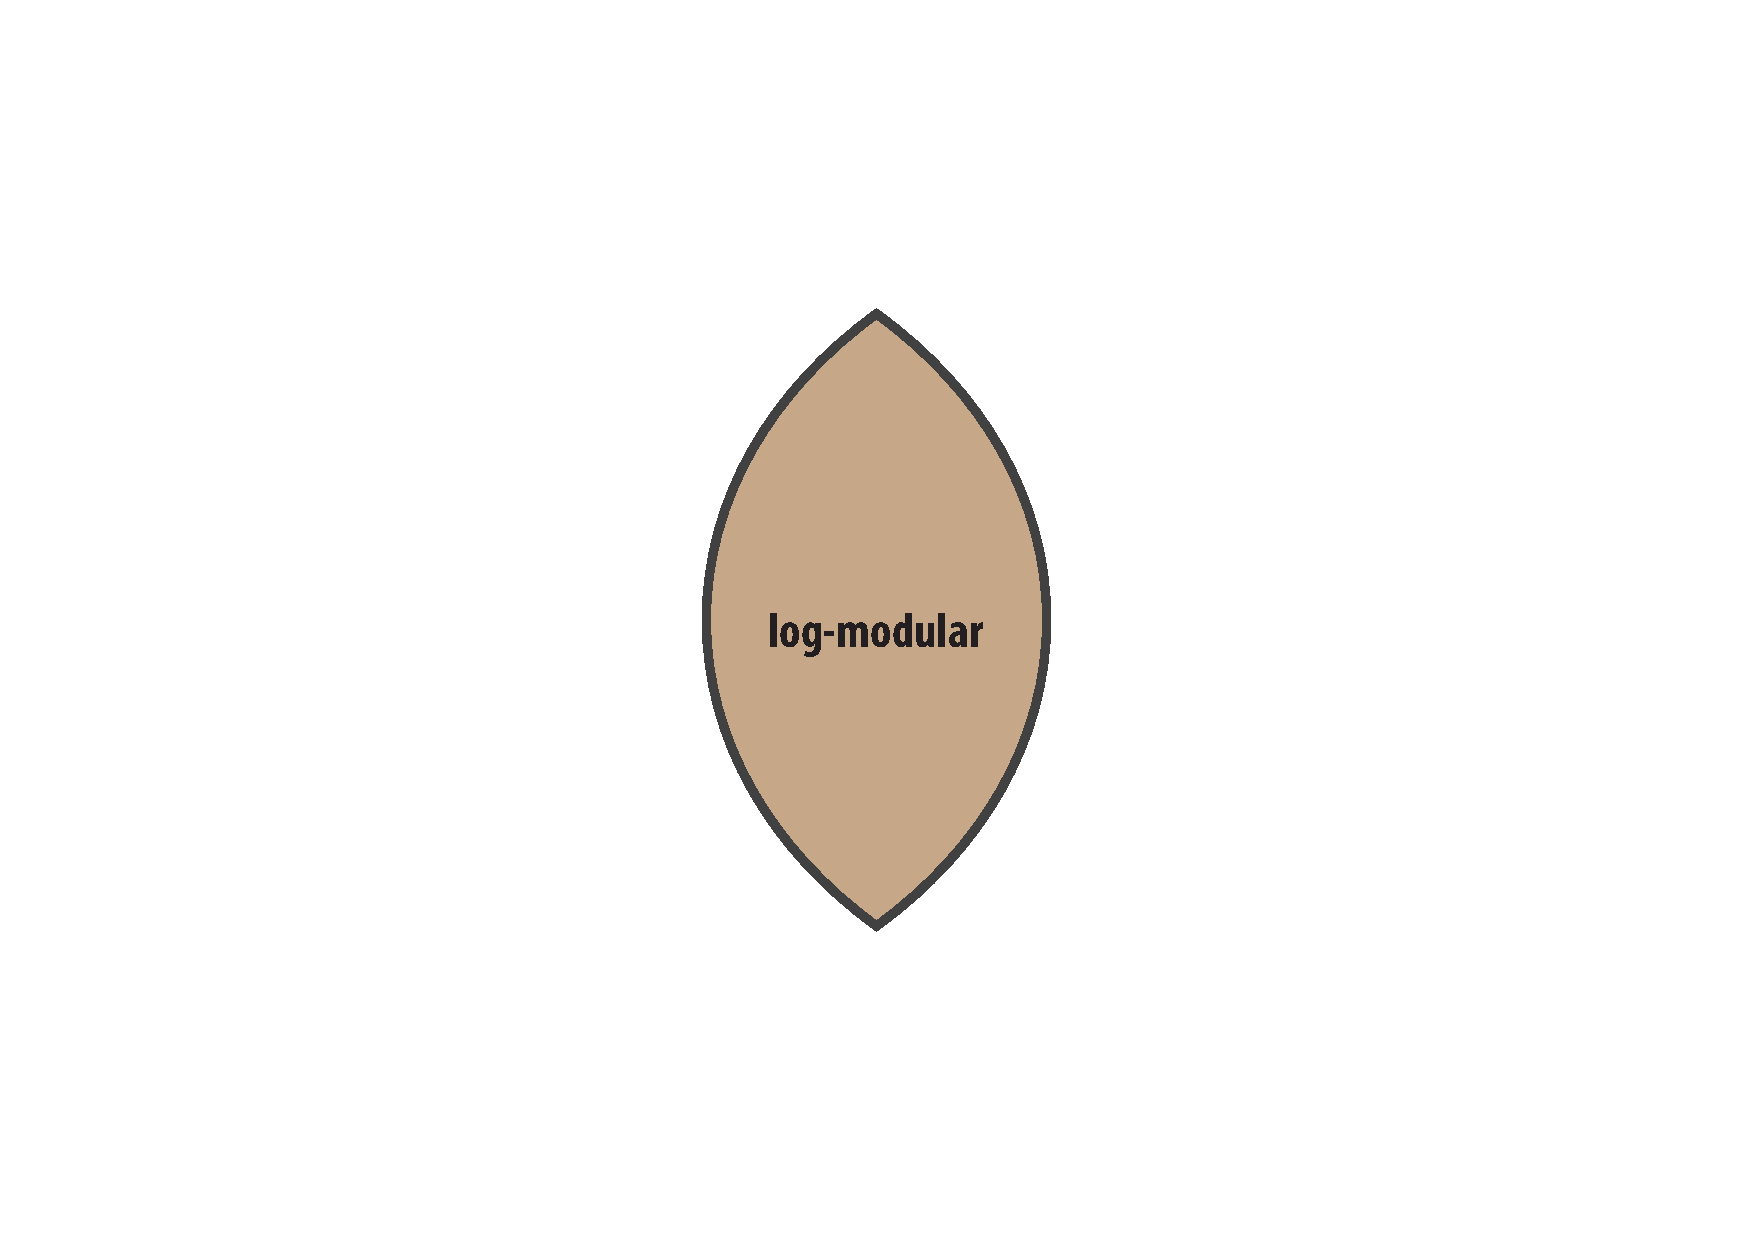
\includegraphics[width=4.3in]{figures/venn01.pdf}
\end{frame}

\begin{frame}{Landscape of Models}
\centering
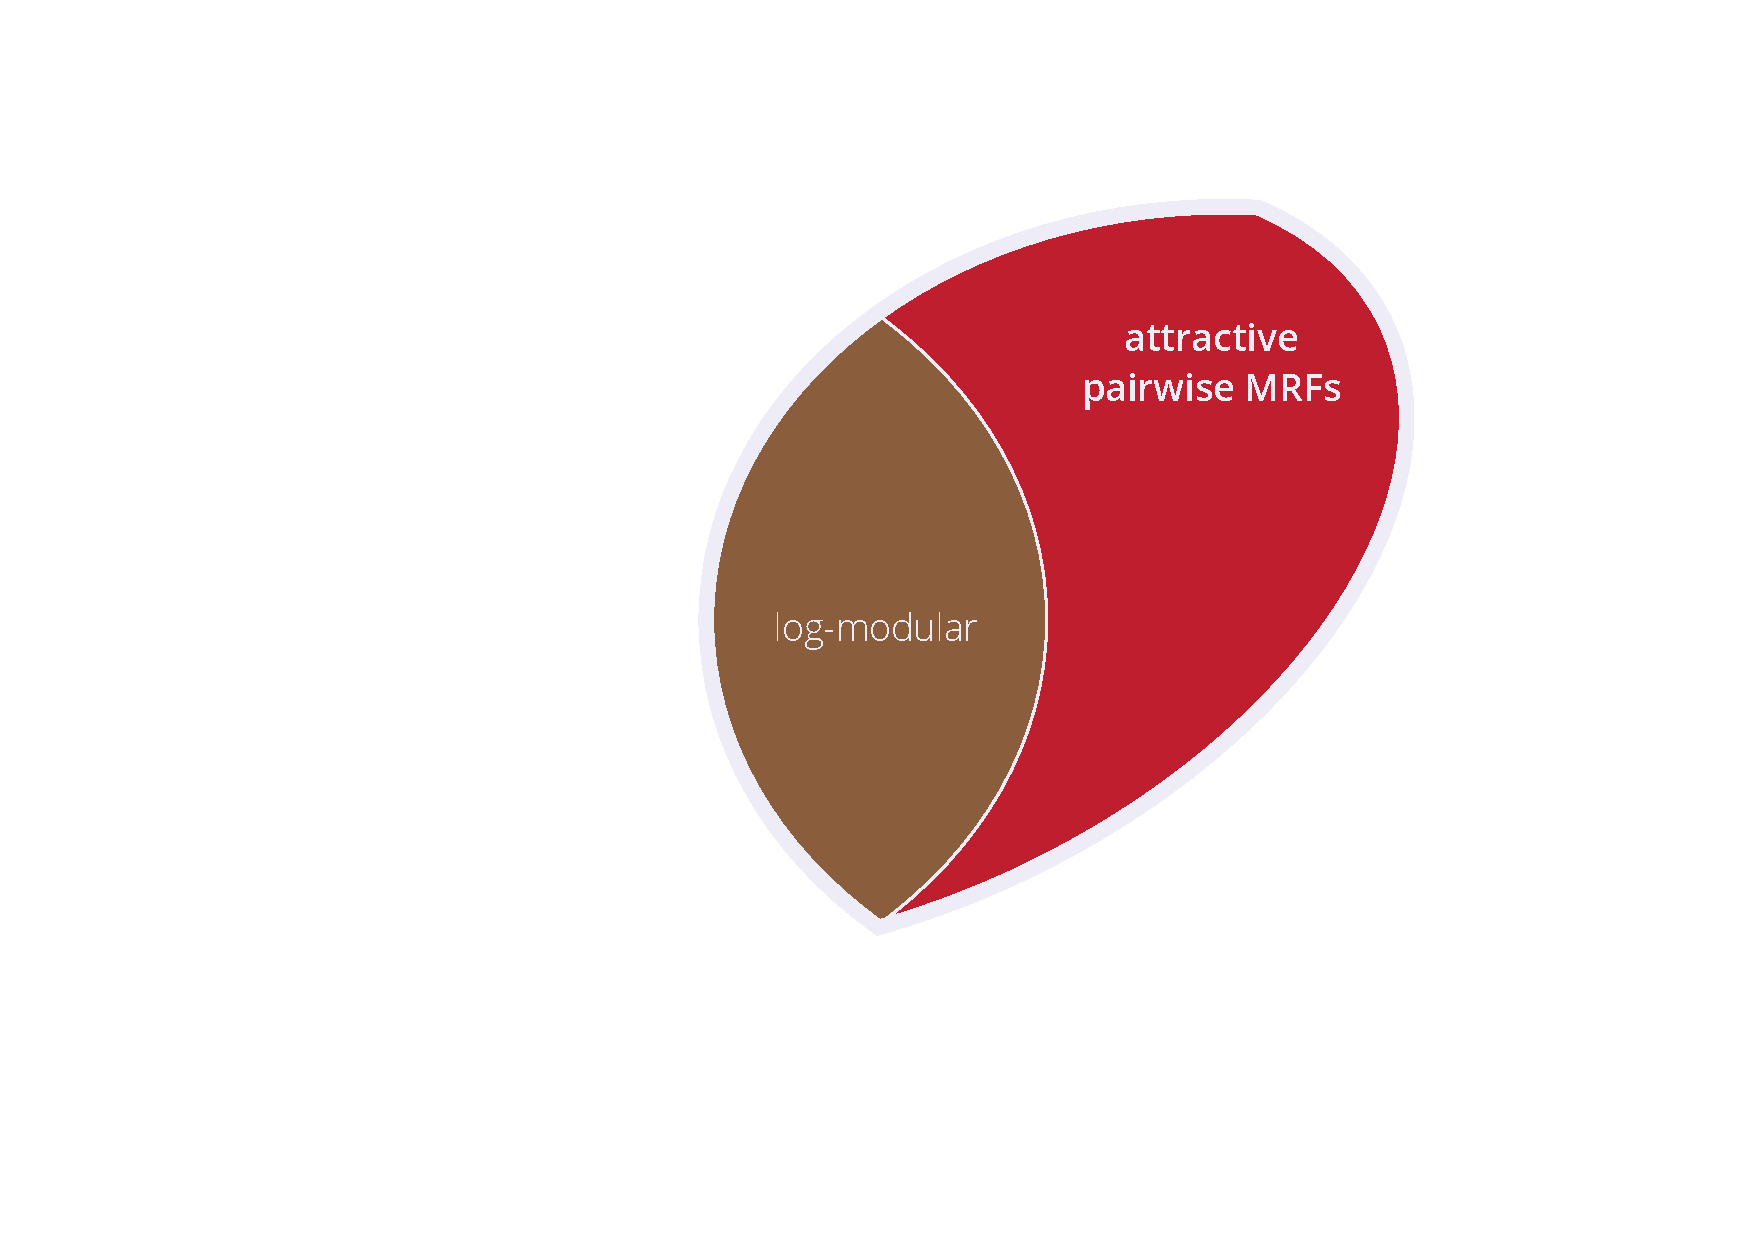
\includegraphics[width=4.3in]{figures/venn02.pdf}
\end{frame}

\begin{frame}{Landscape of Models}
\centering
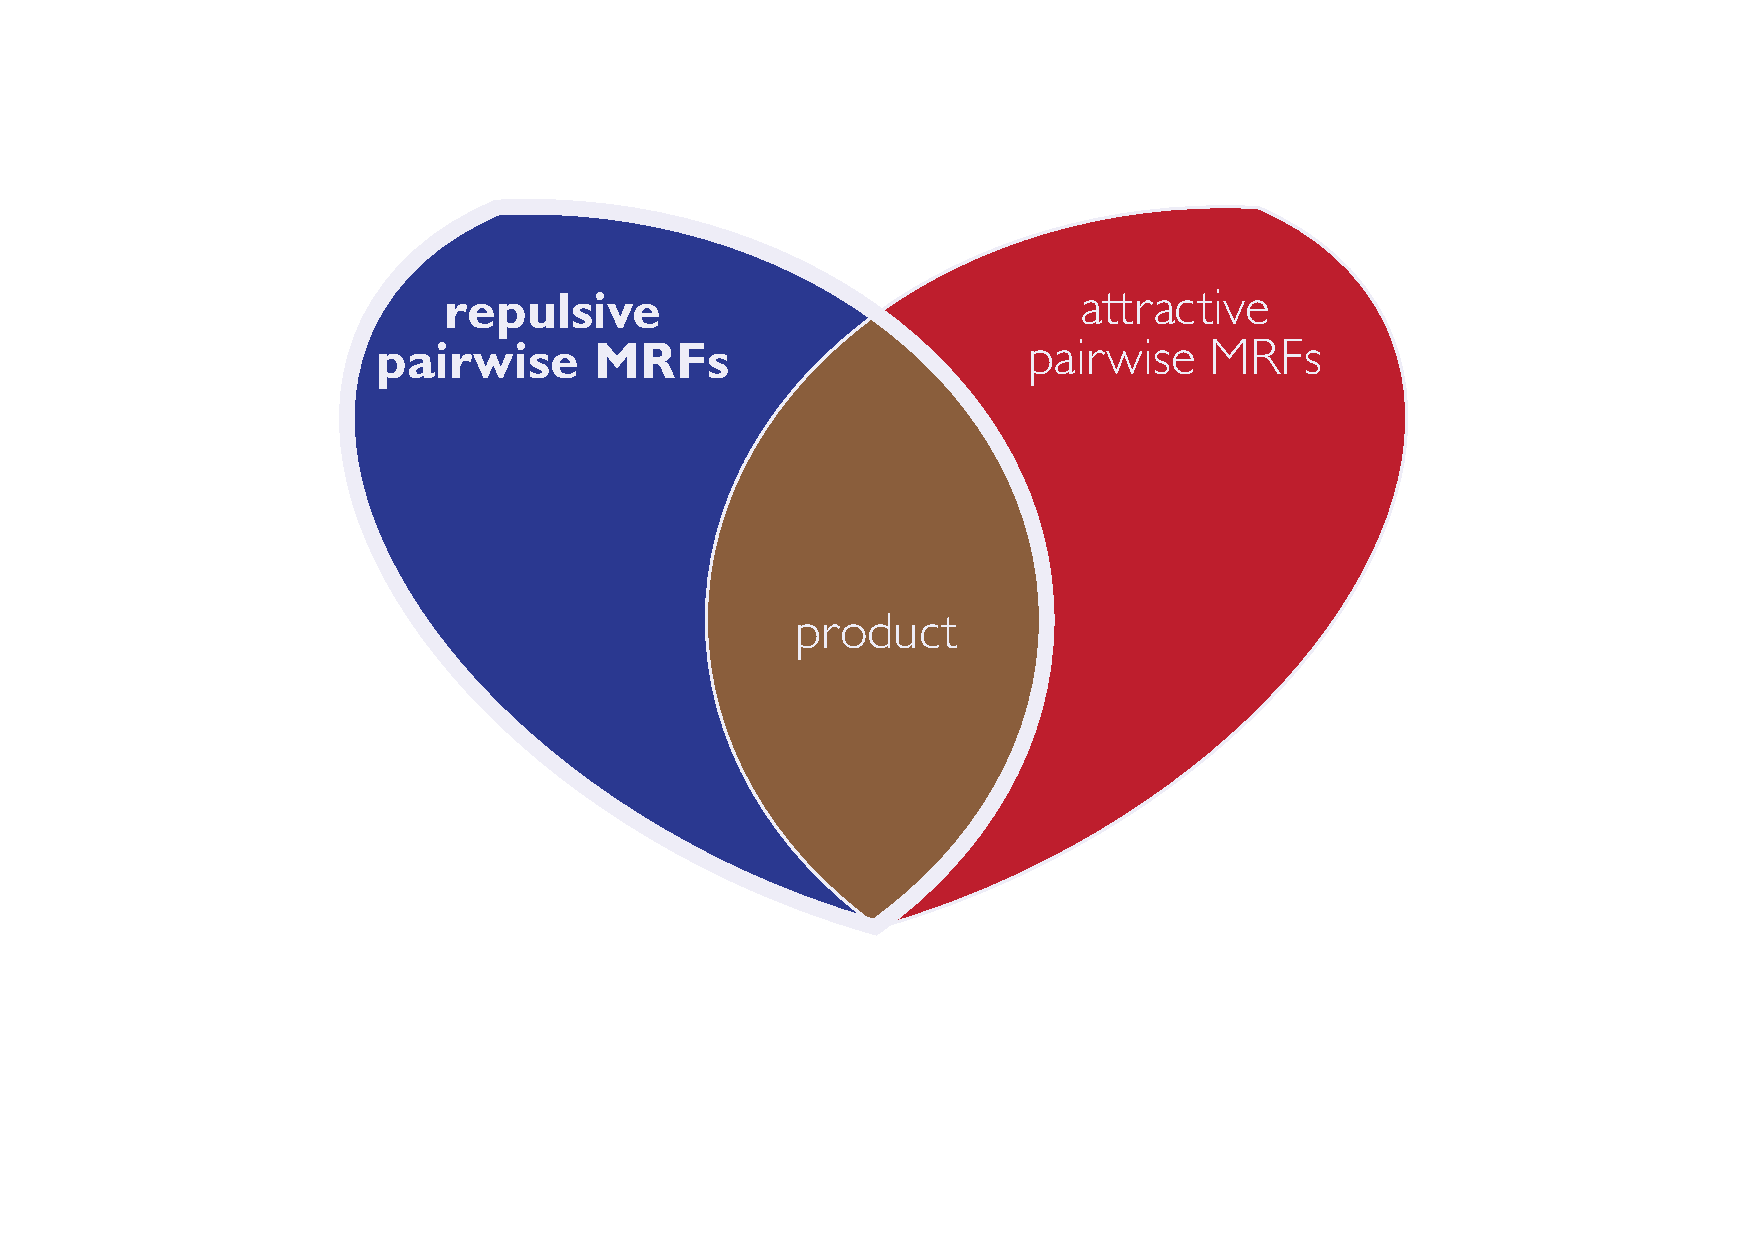
\includegraphics[width=4.3in]{figures/venn03.pdf}
\end{frame}

\begin{frame}{Landscape of Models}
\centering
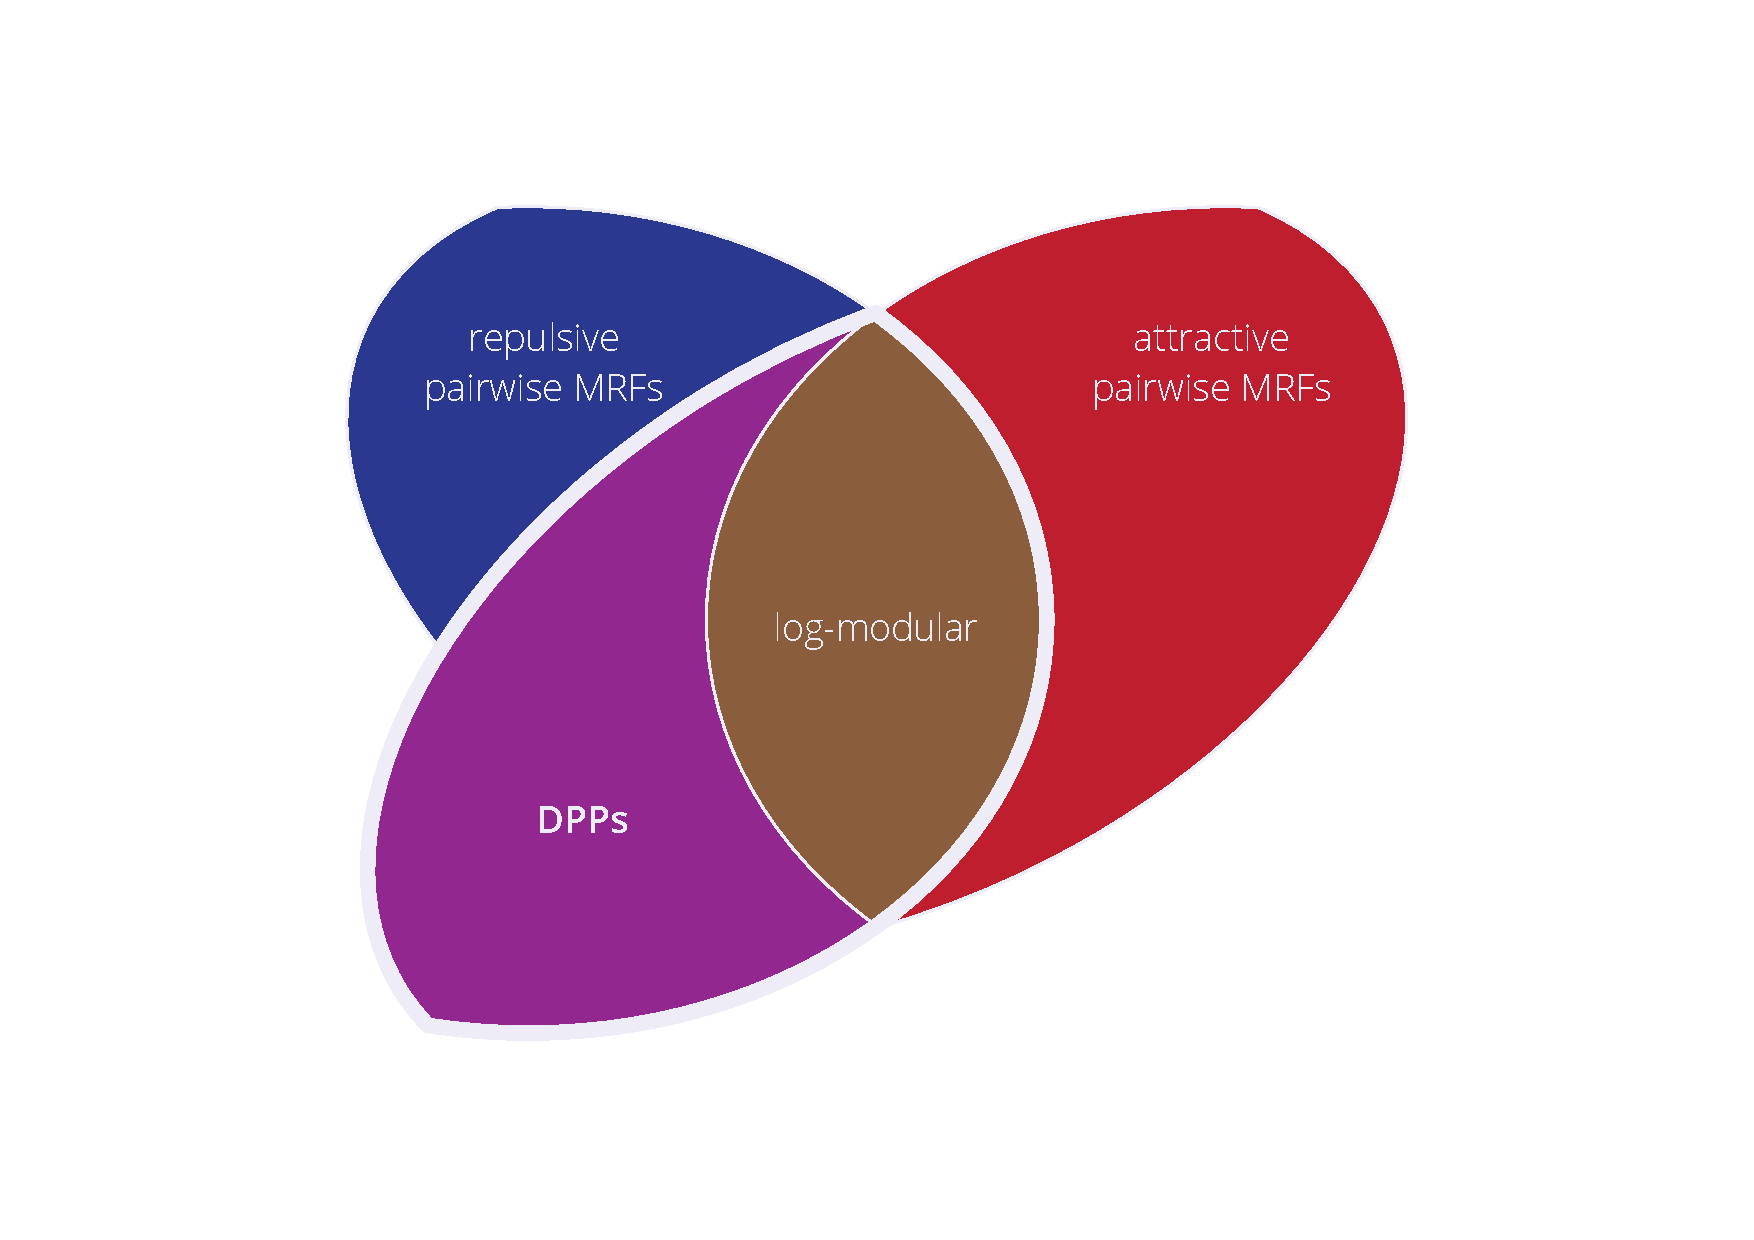
\includegraphics[width=4.3in]{figures/venn04.pdf}
\end{frame}

\begin{frame}{Landscape of Models}
\centering
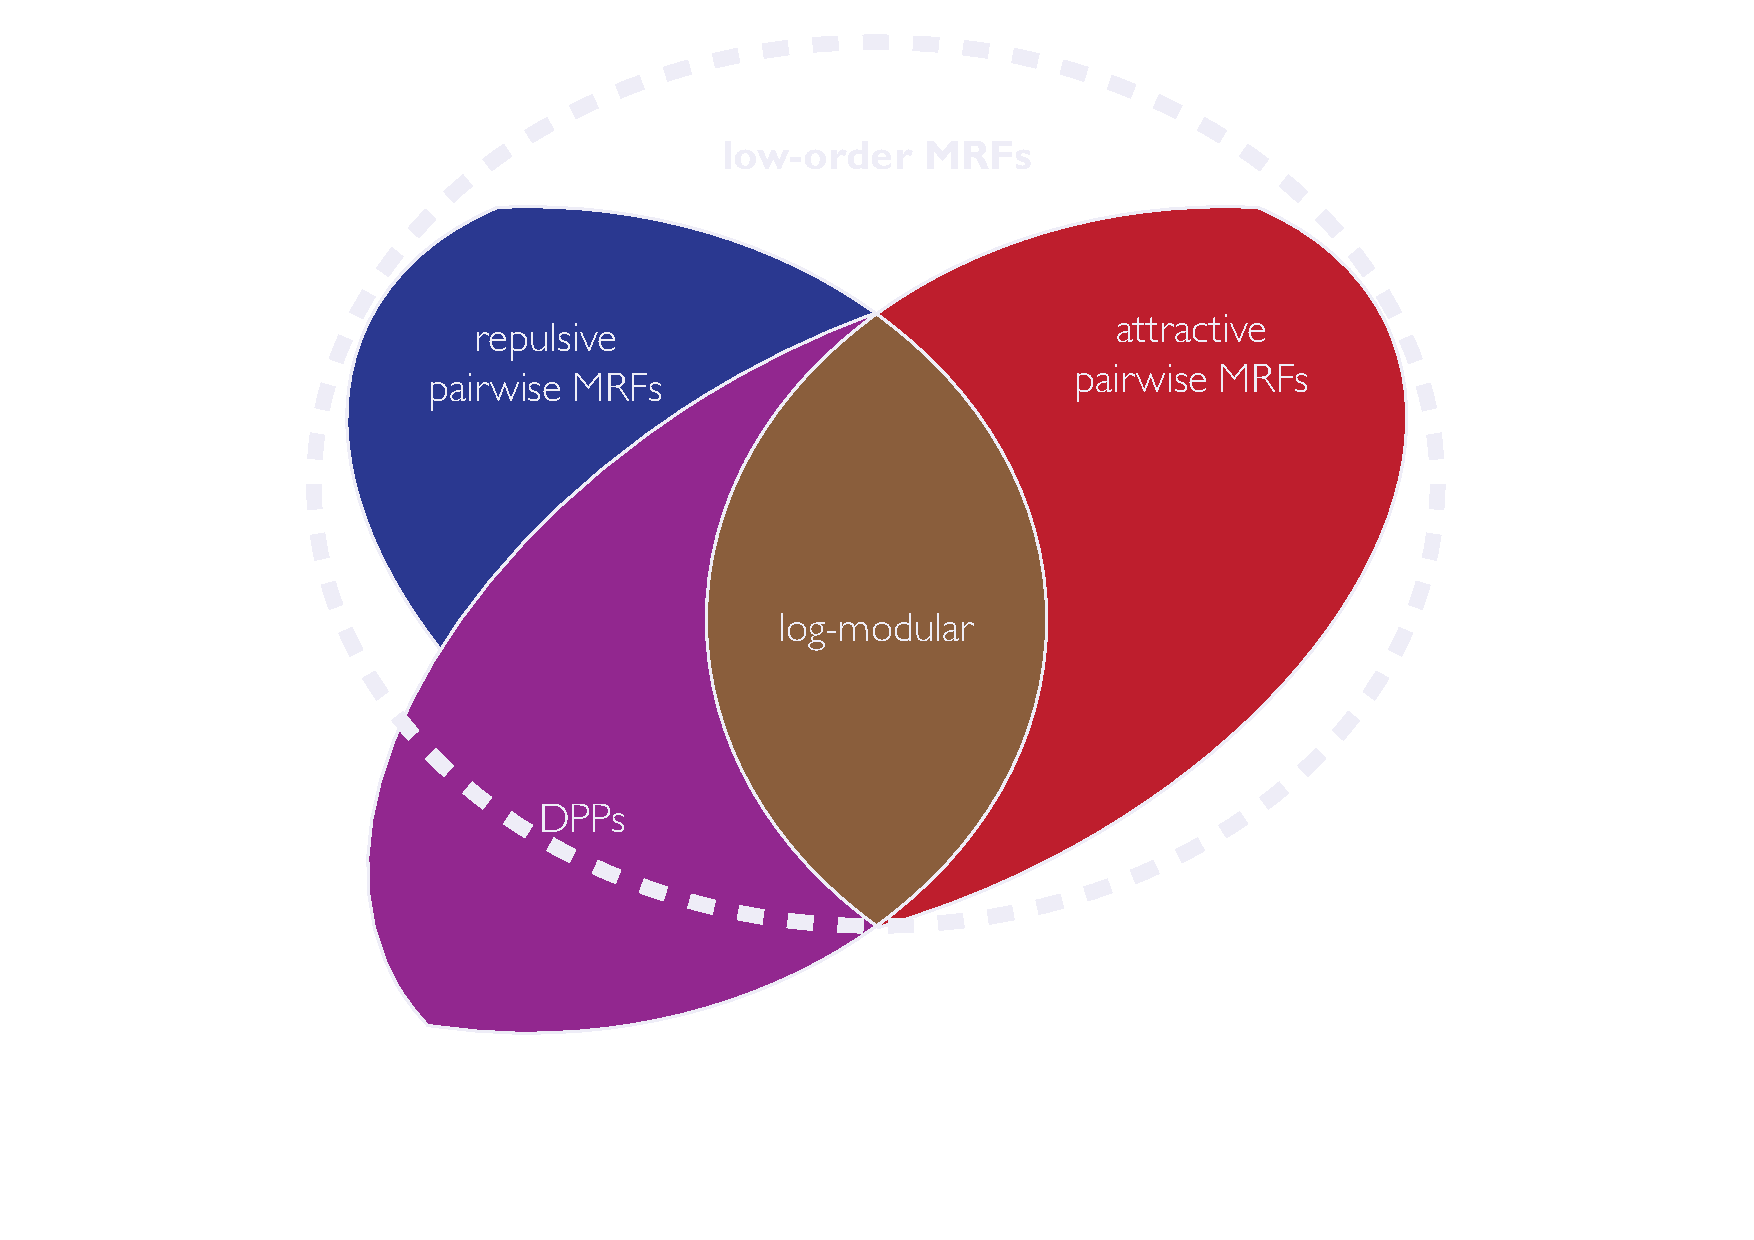
\includegraphics[width=4.3in]{figures/venn05.pdf}
\end{frame}

\begin{frame}{Landscape of Models}
\centering
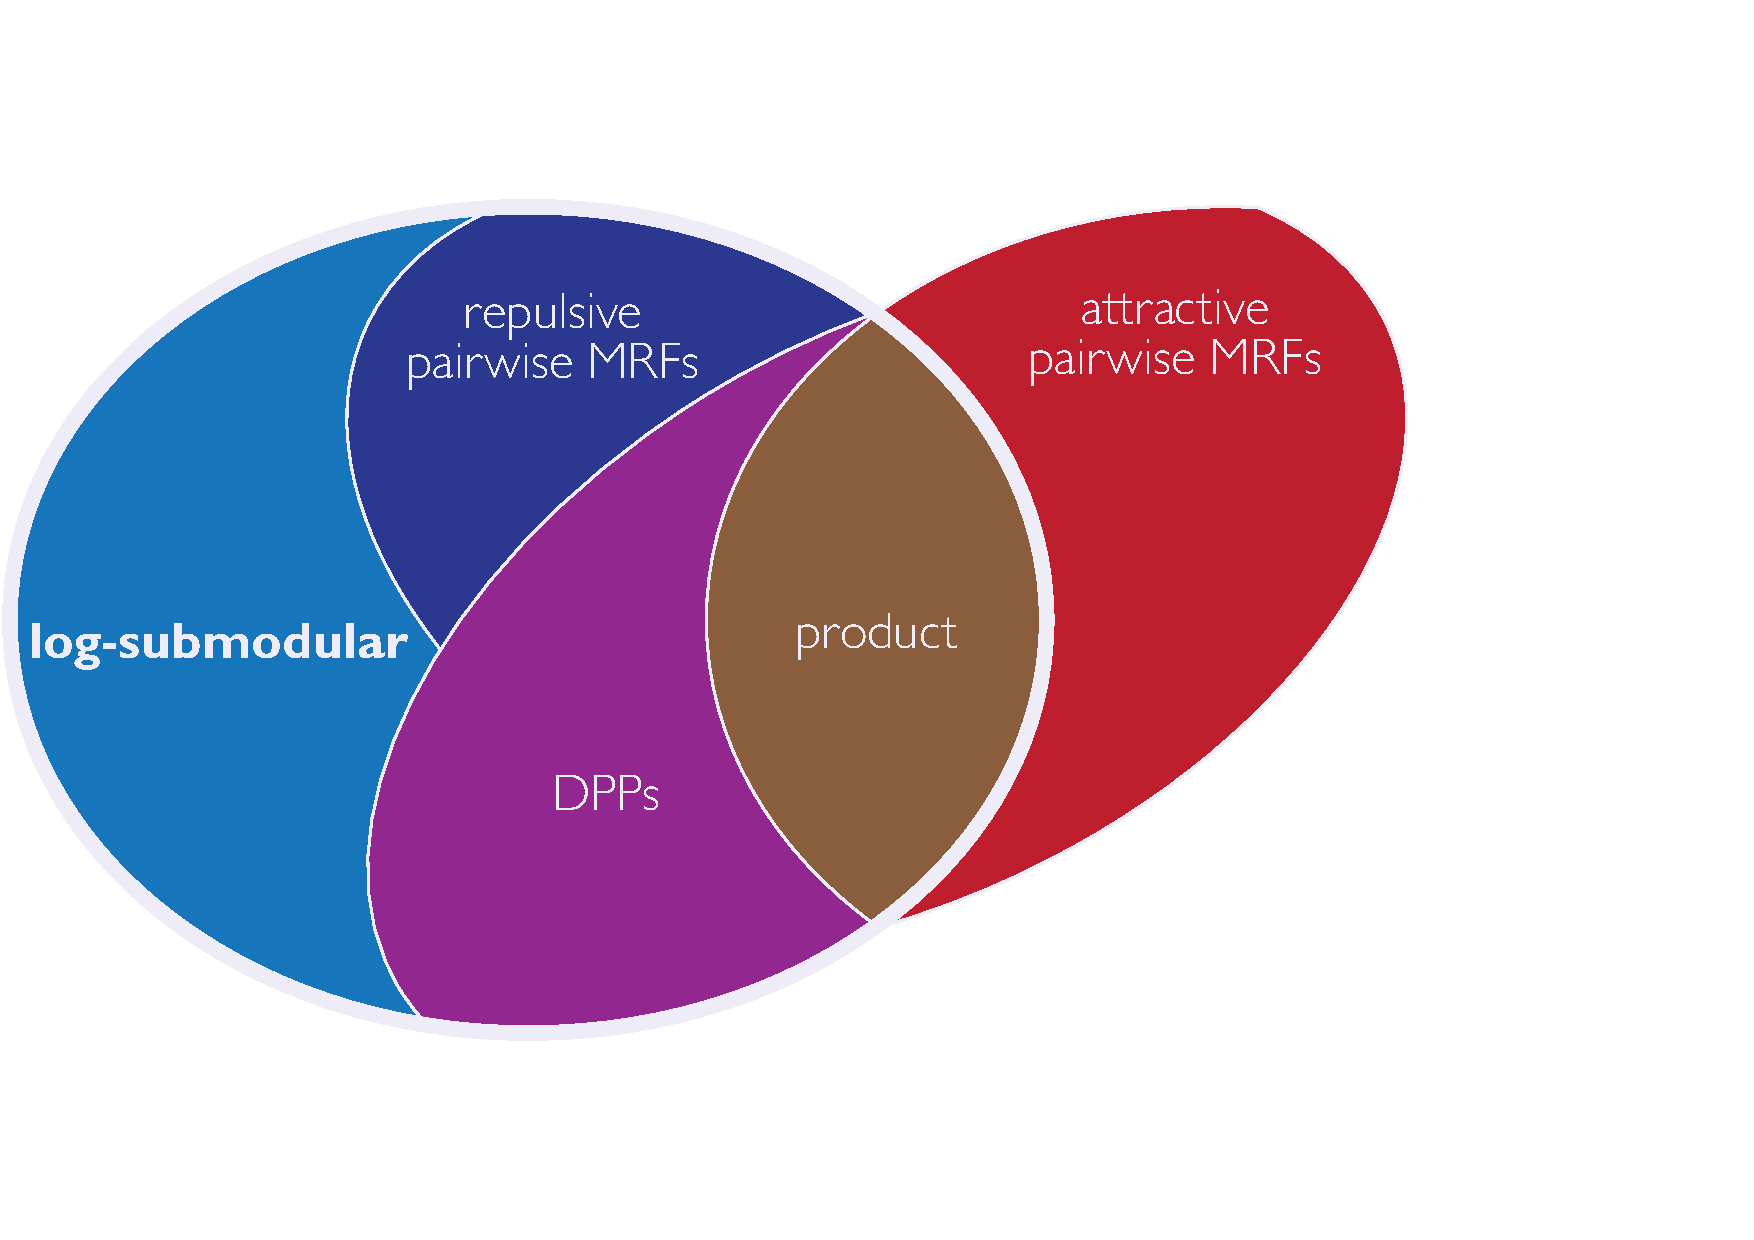
\includegraphics[width=4.3in]{figures/venn06.pdf}
\end{frame}

\begin{frame}{Landscape of Models}
\centering
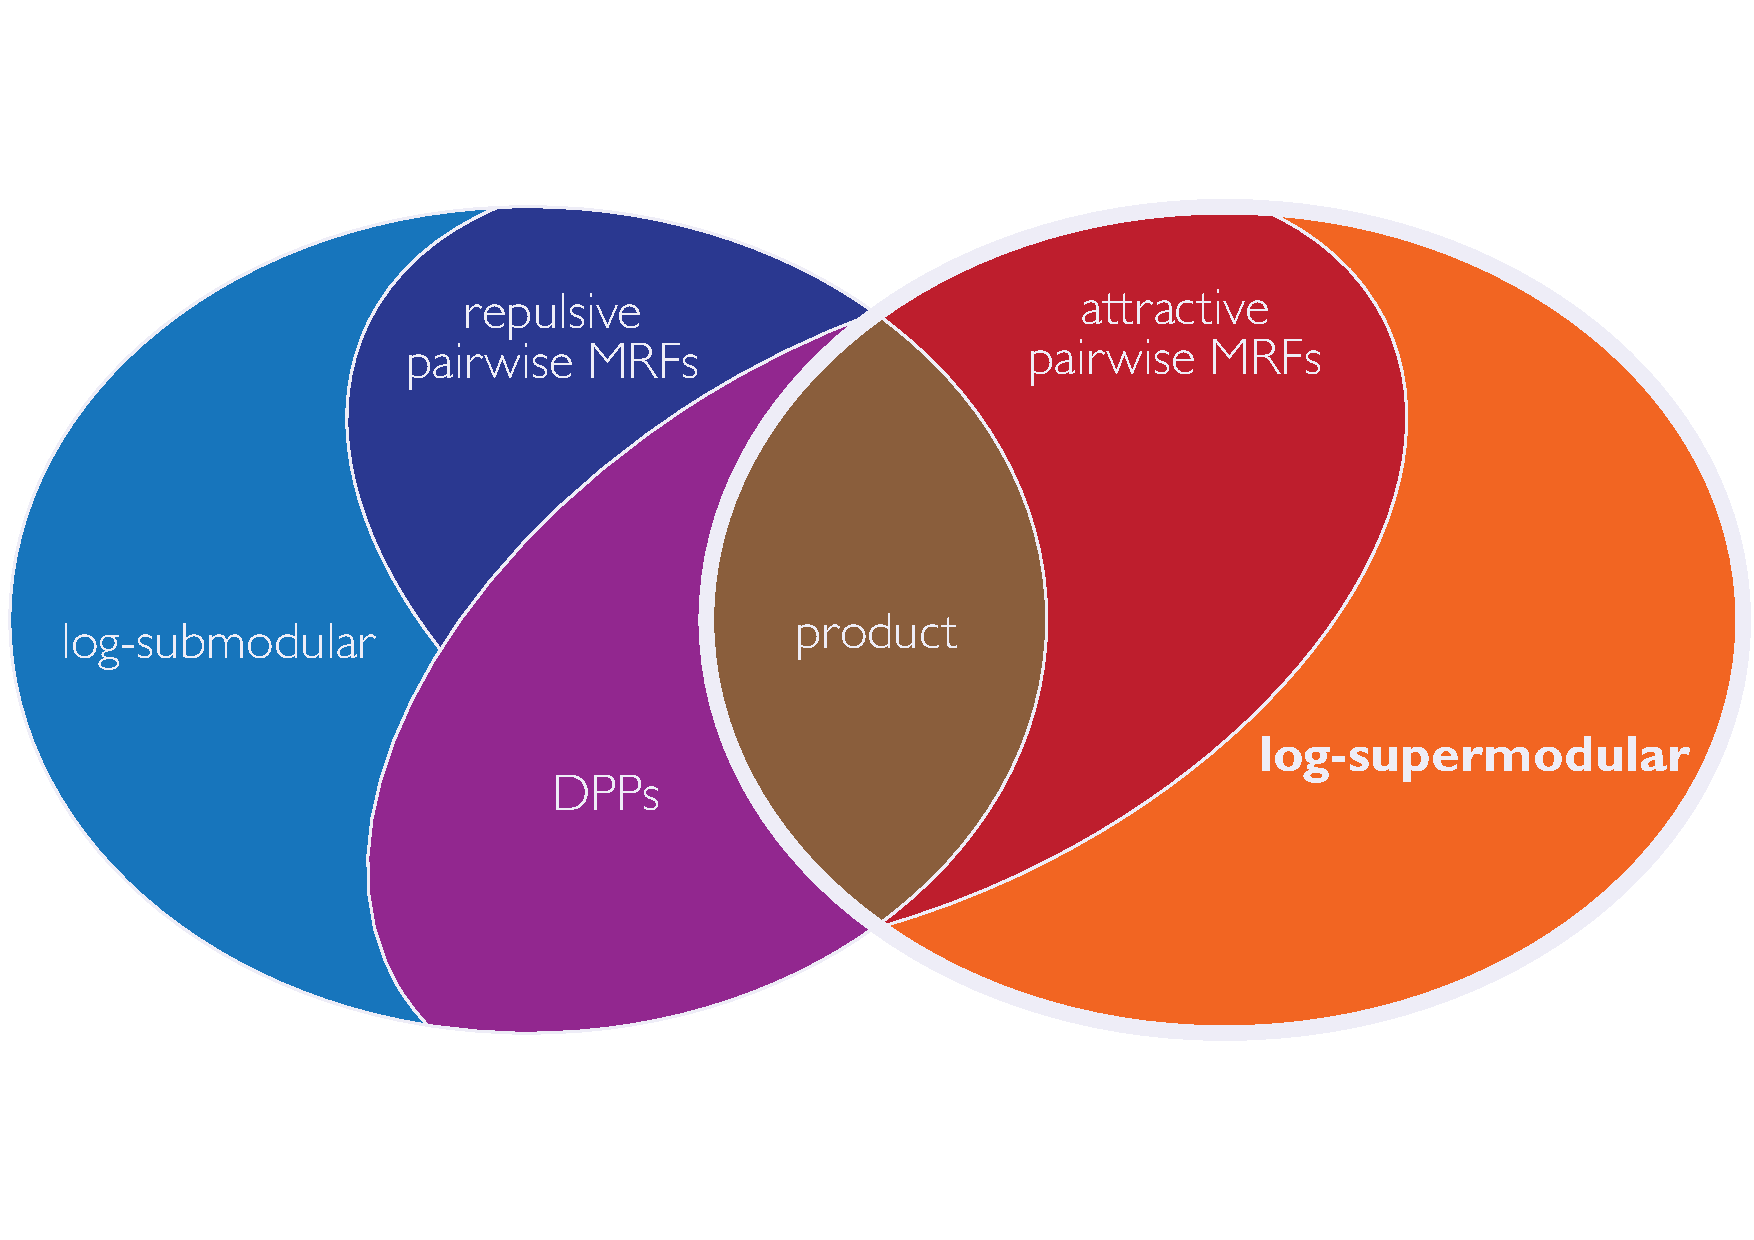
\includegraphics[width=4.3in]{figures/venn07.pdf}
\end{frame}

\begin{frame}{Landscape of Models}
\centering
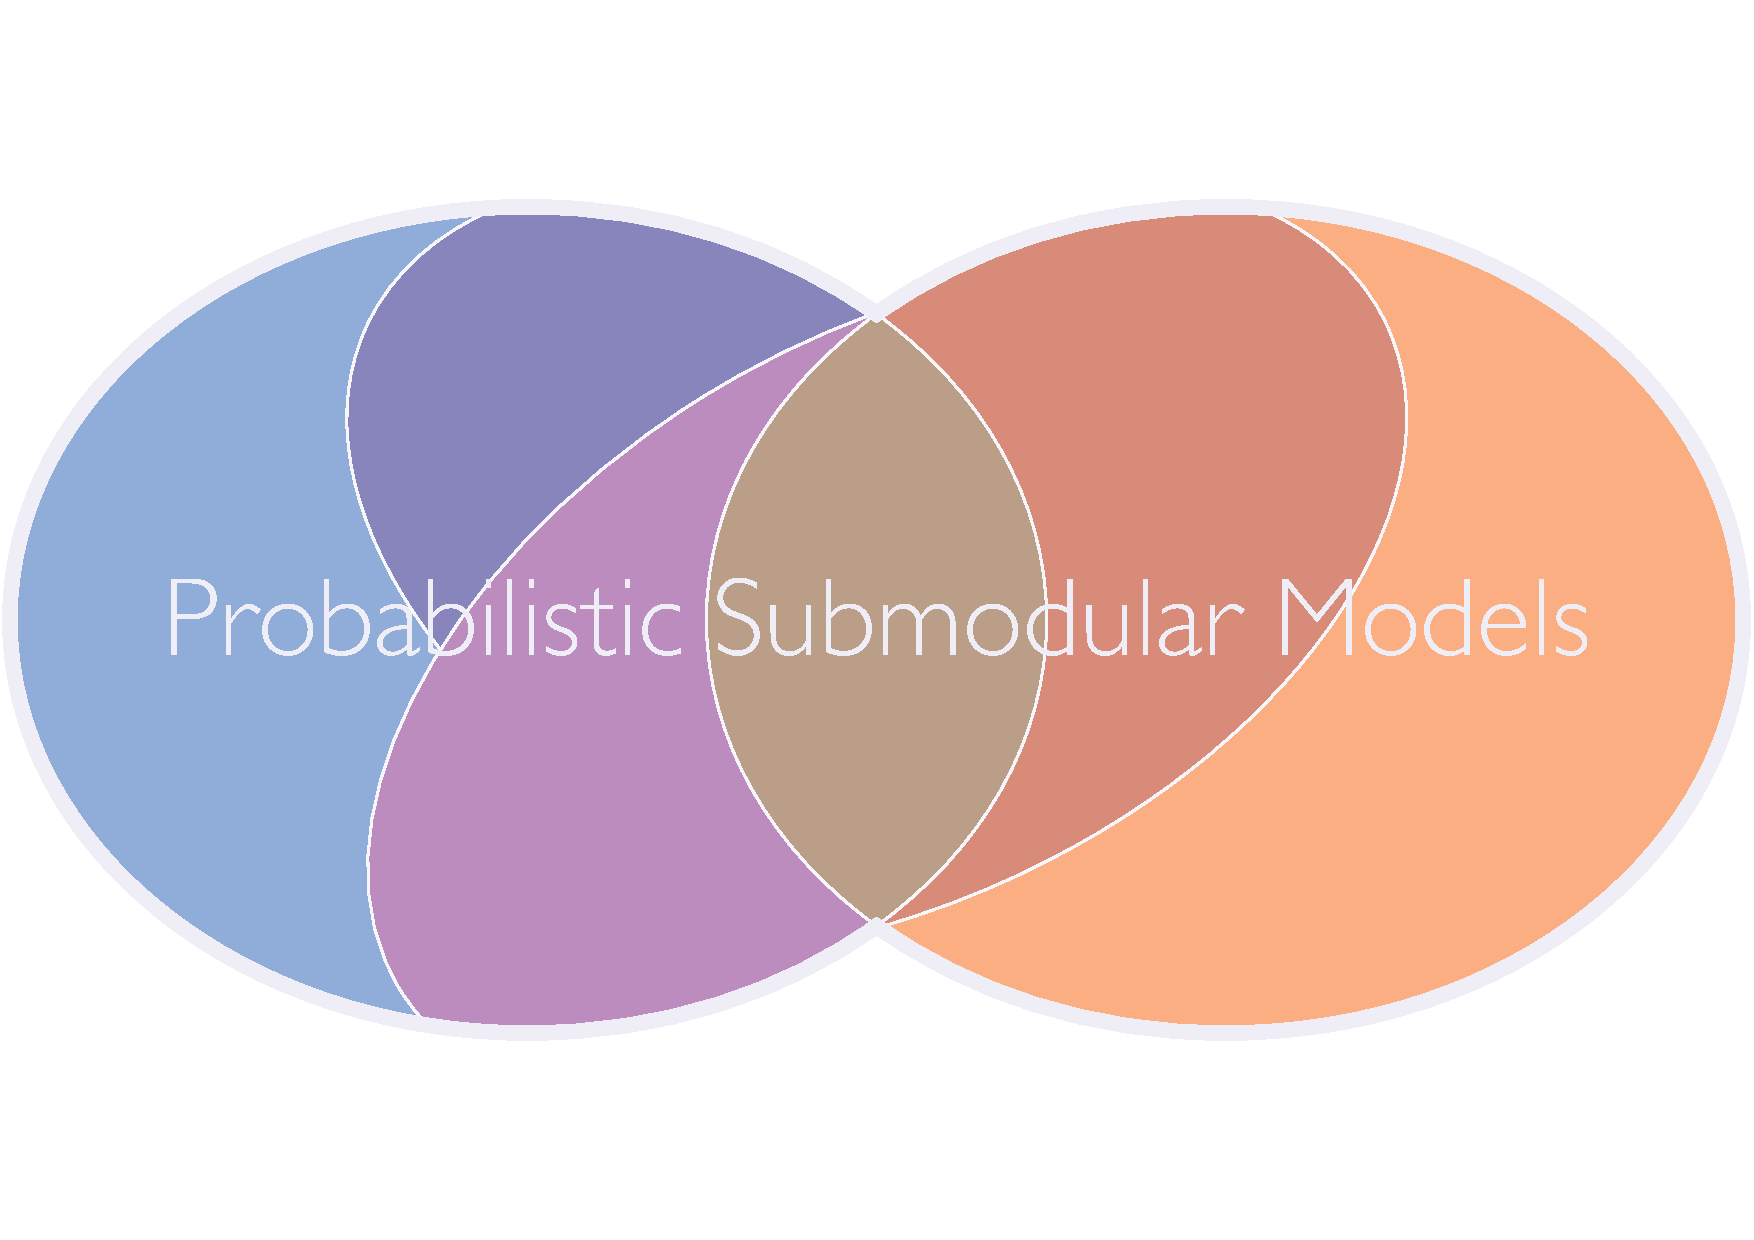
\includegraphics[width=4.3in]{figures/venn08.pdf}
\end{frame}

\end{document}
